\section{チャレンジ課題1}\label{section:challenge1}
\begin{itembox}{チャレンジ課題1}
  主成分分析,多クラスフィッシャー判別分析を実装せよ.
  また,3 クラス,4 次元の iris データセット iris.txt に
  主成分分析とフィッシャー判別分析をそれぞれ適応して 1 次元に
  次元削減し図示せよ.
  次元削減後のクラス間デー タの分離の違いを確認せよ.
  なお iris データセットの各行はデータのインデックス,
  第 5 列はクラス番号(1,2, 3 クラス)を示している.
  各クラス 50 サンプル合計 150 サンプルとなる.
\end{itembox}

主成分分析とフィッシャー線形判別による特徴空間の
変換結果を~\ref{fig:challenge1}に示す.

PCAに比べFisherLDAではクラス1とクラス2,3とのクラス間分散が大きくなり,
クラス3のクラス内分散が小さくなっていることがわかる.
また,クラス2,3の重なりもFisherLDAの方が小さくなっている.


\begin{figure}[htbp]
  \centering
  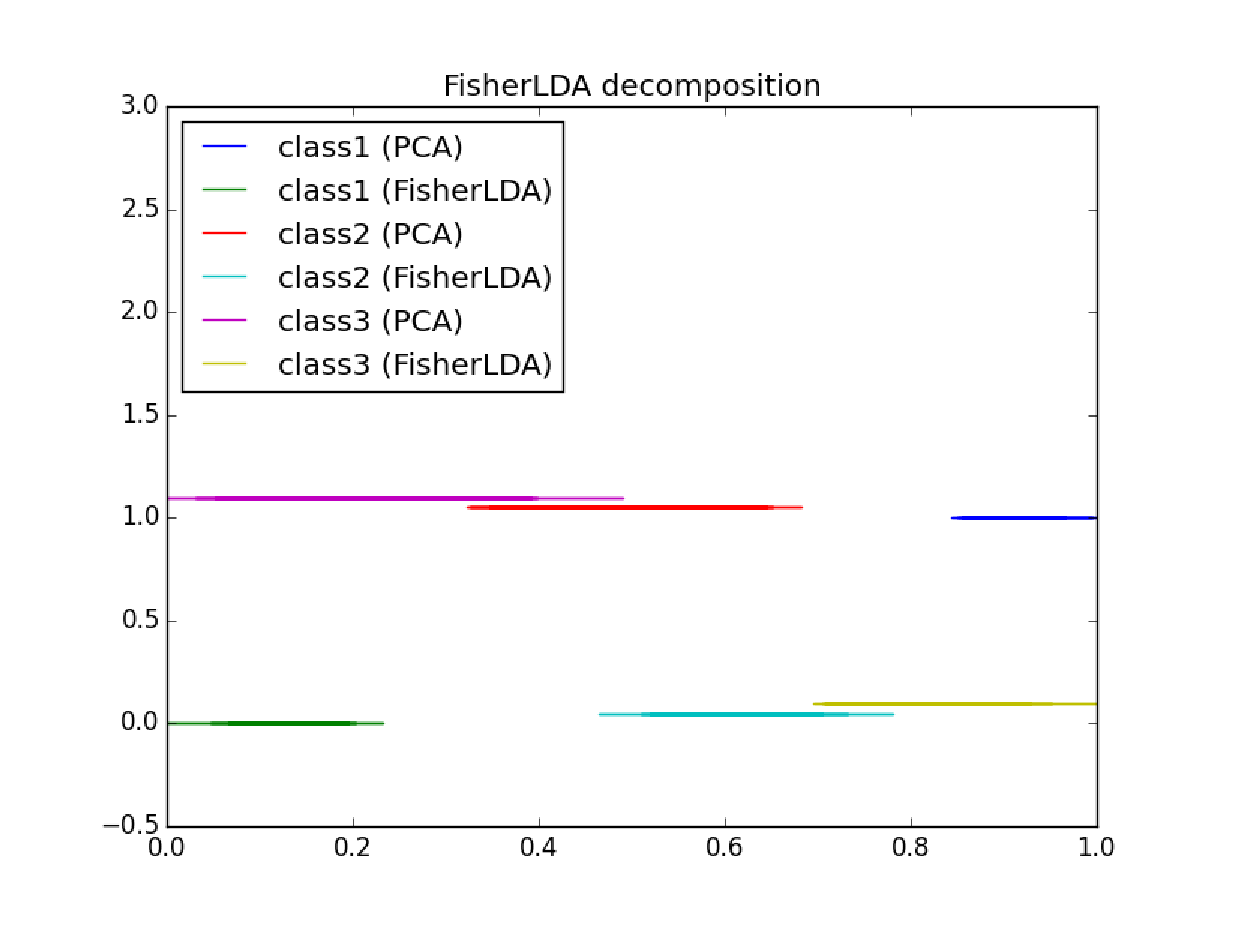
\includegraphics[width=0.7\textwidth]{./assets/challenge1_plot_20150210_050430.eps}
  \caption{PCAとFisherLDAによる特徴空間の変換(データ:iris.txt)}
  \label{fig:challenge1}
\end{figure}